\documentclass[10pt,a4paper]{amsart}
\usepackage[margin=19mm]{geometry}
\usepackage{amsmath,amssymb,mathtools}
\usepackage[scr=rsfs,cal=euler]{mathalfa}
\usepackage{xfrac}
\usepackage[unicode,hidelinks,bookmarks=false]{hyperref}
\newcommand{\ie}{i.e.\ }
\newcommand{\cf}{cf.\ }
\newcommand{\resp}{respectively\ }
\newcommand{\Subsection}{\subsection}
\providecommand{\nobreakdash}{\nobreak\hbox{-}}
\setlength{\emergencystretch}{2em}
\multlinegap0pt
\usepackage{tikz}
\usepackage{amssymb}
\usepackage{mathtools}
\usepackage[all]{xy}
\newtheorem{theorem}{Theorem}
\title{Vassiliev invariants for virtual knotoids}
\author{Siqi Ding, Xiaobo Jin, Fengchun Lei, Fengling Li, Andrei Vesnin}
\date{Source: arXiv:2511.20269v3 (CC BY 4.0)}
\begin{document}
\maketitle

\noindent\emph{Source and licence.} Vassiliev invariants for virtual knotoids. Version arXiv:2511.20269v3 (CC BY 4.0), distributed by arXiv under the Creative Commons Attribution 4.0 International licence, http://creativecommons.org/licenses/by/4.0/, as recorded in the arXiv licence metadata for this exact version and shown on the abstract page https://arxiv.org/abs/2511.20269v3. Full licence notice: \texttt{licenses/arxiv-2511.20269-CC-BY-4.0.txt}.\par\smallskip

\noindent\textit{Editorial scope.} Counted unit: the article's theorem th3.1 (source0.tex lines 1015--1017). The article's complete original proof of it is delivered with it (source0.tex lines 1020--1319, one \texttt{proof} environment of 300 lines). No mathematics is written, repaired or re-derived: the statement and the proof are the article's own lines, in the article's own notation, and no retained line is substituted or re-flowed.  No further source-local context is needed: every cross-reference of every retained line resolves inside the two delivered spans.  Nothing was omitted from any retained span, so the package carries no omission record.  No retained line contains a citation, so the wrapper carries no bibliography and no bibliography entry.  The retained lines contain the article's own diagram code, which the wrapper typesets with the standard tikz packages; no image file is delivered and the package declares no asset dependency.  Editorial formatting only, in addition: an AMS \texttt{amsart} preamble that restates the article's own declarations and macros used by the retained lines, namely the environments \texttt{theorem} on separate counters, together with the standard packages those lines need.  The retained environments print in this document as Theorem 1 in order of appearance, whereas the article prints the same items with the numbering of its own full document.  The complete native source of the article as distributed in the arXiv e-print for this exact version is bundled unchanged as \texttt{sources/189776/source0.tex}.
\begin{theorem}\label{th3.1}
Let $D$ be a virtual knotoid diagram. Then $\mathcal{F} (D)$ is a virtual knotoid invariant.
\end{theorem}

\begin{proof} 	
Consider the behavior of $\mathcal{F} (D)$ under moves $\Omega_1$, $\Omega_2$, $\Omega_3$ and $\Omega^m_3$.
	
(1) $\Omega_1$-move.   
Let $D$ and $E$ be virtual knotoid diagrams related by an $\Omega_1$-move, and $c_* \in D$ be the classical crossing  involved in $\Omega_1$. It is clear from Fig.~\ref{fig15} that $[\overline{D_{c_*}} ]= [\overline{E}] = [\overline{D}]$ and $w(E) = w(D) - w_D(c_*)$. Notice that if a classical crossing $c \in D$ is not involved in $\Omega_1$-move then $w_D(c)=w_E(c)$, $[\overline{D_c}] = [\overline{E_c}]$. 

\begin{figure}[!htb]
\begin{center}
\tikzset{every picture/.style={line width=1.0pt}}
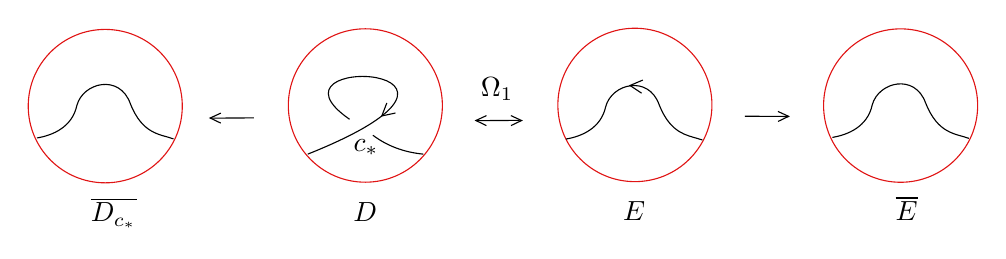
\begin{tikzpicture}[x=0.75pt,y=0.75pt,yscale=-0.8,xscale=0.8]
\draw  [color={rgb, 255:red, 224; green, 20; blue, 20 }  ,draw opacity=1 ] (198.08,107.47) .. controls (198.08,81.96) and (218.85,61.28) .. (244.47,61.28) .. controls (270.09,61.28) and (290.86,81.96) .. (290.86,107.47) .. controls (290.86,132.98) and (270.09,153.67) .. (244.47,153.67) .. controls (218.85,153.67) and (198.08,132.98) .. (198.08,107.47) -- cycle ;
\draw    (234.97,115.78) .. controls (176.44,75.28) and (345.29,82.56) .. (209.8,136.77) ;
\draw    (249.01,125.4) .. controls (257.21,131.52) and (267.16,135.6) .. (279.45,136.77) ;
\draw  [color={rgb, 255:red, 224; green, 20; blue, 20 }  ,draw opacity=1 ] (41.44,107.85) .. controls (41.44,82.33) and (62.21,61.65) .. (87.83,61.65) .. controls (113.45,61.65) and (134.22,82.33) .. (134.22,107.85) .. controls (134.22,133.36) and (113.45,154.04) .. (87.83,154.04) .. controls (62.21,154.04) and (41.44,133.36) .. (41.44,107.85) -- cycle ;
\draw    (128.95,127.6) .. controls (121.05,124.69) and (110.37,125.13) .. (102.91,106.33) .. controls (96.47,88.26) and (74.46,93.5) .. (70.72,107.5) .. controls (67.91,120.52) and (56.16,125.48) .. (46.72,127.02) ;
\draw    (177.4,114.94) -- (151,115.09) ;
\draw   (157.43,112.06) -- (151.03,115.01) -- (157.38,118.07) ;
\draw  [color={rgb, 255:red, 224; green, 20; blue, 20 }  ,draw opacity=1 ] (360.41,107.14) .. controls (360.41,81.63) and (381.18,60.94) .. (406.8,60.94) .. controls (432.43,60.94) and (453.2,81.63) .. (453.2,107.14) .. controls (453.2,132.65) and (432.43,153.33) .. (406.8,153.33) .. controls (381.18,153.33) and (360.41,132.65) .. (360.41,107.14) -- cycle ;
\draw  [color={rgb, 255:red, 224; green, 20; blue, 20 }  ,draw opacity=1 ] (520.44,107.51) .. controls (520.44,82) and (541.21,61.32) .. (566.83,61.32) .. controls (592.45,61.32) and (613.22,82) .. (613.22,107.51) .. controls (613.22,133.03) and (592.45,153.71) .. (566.83,153.71) .. controls (541.21,153.71) and (520.44,133.03) .. (520.44,107.51) -- cycle ;
\draw    (607.95,127.27) .. controls (600.05,124.36) and (589.37,124.8) .. (581.91,106) .. controls (575.47,87.93) and (553.46,93.17) .. (549.72,107.16) .. controls (546.91,120.19) and (535.16,125.14) .. (525.72,126.69) ;
\draw    (473,113.93) -- (499.4,114.09) ;
\draw   (492.97,111.06) -- (499.37,114.02) -- (493.02,117.08) ;
\draw    (447.45,128.27) .. controls (440.72,125.79) and (431.97,125.74) .. (424.91,114.14) .. controls (423.68,112.13) and (422.51,109.77) .. (421.41,107) .. controls (414.97,88.93) and (392.96,94.17) .. (389.22,108.16) .. controls (386.41,121.19) and (374.66,126.14) .. (365.22,127.69) ;
\draw    (337.4,116.44) -- (311,116.59) ;
\draw   (317.43,113.56) -- (311.03,116.51) -- (317.38,119.57) ;
\draw   (332.13,113.56) -- (338.54,116.52) -- (332.19,119.58) ;
\draw   (262.58,112.01) -- (254.39,113.77) -- (257.38,105.98) ;
\draw   (410.82,100.07) -- (403.86,95.42) -- (411.58,92.16) ;
\draw (235.85,126.36) node [anchor=north west][inner sep=0.75pt]  [font=\normalsize]  {$c_{*}$};
\draw (235.75,164.07) node [anchor=north west][inner sep=0.75pt]    {$D$};
\draw (77.6,161.3) node [anchor=north west][inner sep=0.75pt]    {$\overline{D_{c_{*}}}$};
\draw (398.08,163.74) node [anchor=north west][inner sep=0.75pt]    {$E$};
\draw (562.2,160.57) node [anchor=north west][inner sep=0.75pt]    {$\overline{E}$};
\draw (312.4,89) node [anchor=north west][inner sep=0.75pt]    {$\Omega _{1}$};
\end{tikzpicture}
\caption{$0$-smoothing and flattening related to $\Omega_1$.} \label{fig15}
\end{center}
\end{figure} 
	
Therefore, 
$$
\mathcal{F} (D) = \sum_{c} w_D(c) \, [\overline{D_c}] - w(D) \, [\overline{D}] = \sum_{c \neq c_*} w_D(c) \, [\overline{D_c}] + w_D(c_*) \, [\overline{D_{c_*}}] - w(D) \, [\overline{D}]  ,
$$

and 
\begin{eqnarray*}
\mathcal{F} (E) &= & \sum_c w_E (c) \, [\overline{E_c}] - w (E) \, [\overline{E}]    
=  \sum_{c \neq c_*} w_D (c) \,  [\overline{D_c}] - \Big( w(D) - w_D(c_*) \Big) \, [\overline{E}] \\ 
& = & \sum_{c \neq c_*} w_D(c) \, [\overline{D_c}] + w_D(c_*) \, [\overline{E}] - w(D) \, [\overline{E}]   
=  \sum _ { c\neq c_* } w_D(c) \, [\overline{D_c}] + w_D(c_*) \, [\overline{D_{c_*}}] - w(D) \, [\overline{D}]   
=  \mathcal{F} (D) ,
\end{eqnarray*}

	
(2) $\Omega_2$-move.
	Let $D$ and $E$ be virtual knotoid diagrams related by an $\Omega_2$-move, and $c_1, c_2 \in D$ are classical crossings  involved in $\Omega_2$. It is clear, see Fig.~\ref{fig16}, that $[\overline{D_{c_{1}}}] = [\overline{D_{c_{2}}}]$ and $w_D(c_{1}) = -w_D(c_{2})$. Moreover,  $[\overline{E}] = [\overline{D}]$ and $w(E)=w(D)-w_D(c_{1})-w_D(c_{2})$. Notice that $w_D(c)=w_E(c)$ and $[\overline{D_c}] = [\overline{E_c}]$ if $c$ is a classical crossing not involved in $\Omega_2$ move. 
	\begin{figure}[!htb]
		\begin{center}
			\tikzset{every picture/.style={line width=1.0pt}}
			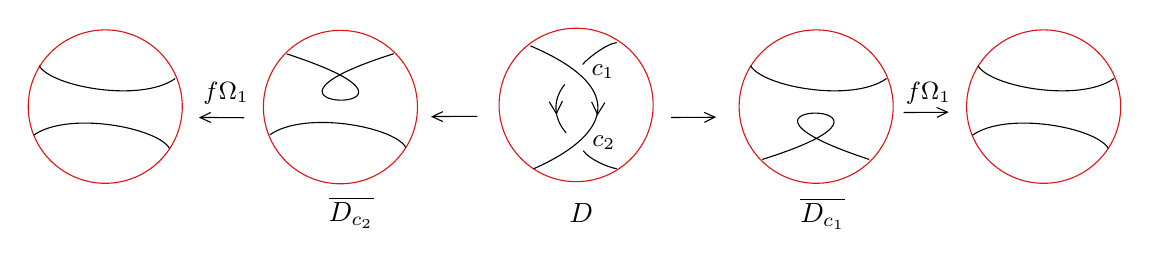
\begin{tikzpicture}[x=0.75pt,y=0.75pt,yscale=-0.8,xscale=0.8]	
				\draw  [color={rgb, 255:red, 224; green, 20; blue, 20 }  ,draw opacity=1 ] (140.08,258.8) .. controls (140.08,233.29) and (160.85,212.61) .. (186.47,212.61) .. controls (212.09,212.61) and (232.86,233.29) .. (232.86,258.8) .. controls (232.86,284.32) and (212.09,305) .. (186.47,305) .. controls (160.85,305) and (140.08,284.32) .. (140.08,258.8) -- cycle ;
				\draw    (504.95,290.33) .. controls (388.95,252.33) and (556.55,253.93) .. (440.55,290.33) ;
				\draw  [color={rgb, 255:red, 224; green, 20; blue, 20 }  ,draw opacity=1 ] (-1.56,258.51) .. controls (-1.56,233) and (19.21,212.32) .. (44.83,212.32) .. controls (70.45,212.32) and (91.22,233) .. (91.22,258.51) .. controls (91.22,284.03) and (70.45,304.71) .. (44.83,304.71) .. controls (19.21,304.71) and (-1.56,284.03) .. (-1.56,258.51) -- cycle ;
				\draw    (128.4,265.21) -- (102,265.05) ;
				\draw   (108.43,268.08) -- (102.03,265.12) -- (108.38,262.06) ;
				\draw  [color={rgb, 255:red, 224; green, 20; blue, 20 }  ,draw opacity=1 ] (282.01,257.51) .. controls (282.01,232) and (302.78,211.32) .. (328.41,211.32) .. controls (354.03,211.32) and (374.8,232) .. (374.8,257.51) .. controls (374.8,283.03) and (354.03,303.71) .. (328.41,303.71) .. controls (302.78,303.71) and (282.01,283.03) .. (282.01,257.51) -- cycle ;
				\draw    (385.57,265.08) -- (411.97,264.94) ;
				\draw   (405.51,261.99) -- (411.94,264.86) -- (405.63,268) ;
				\draw  [color={rgb, 255:red, 224; green, 20; blue, 20 }  ,draw opacity=1 ] (426.58,258.51) .. controls (426.58,233) and (447.35,212.32) .. (472.97,212.32) .. controls (498.59,212.32) and (519.36,233) .. (519.36,258.51) .. controls (519.36,284.03) and (498.59,304.71) .. (472.97,304.71) .. controls (447.35,304.71) and (426.58,284.03) .. (426.58,258.51) -- cycle ;
				\draw    (242.47,264.5) -- (268.87,264.36) ;
				\draw   (248.2,267.55) -- (241.8,264.6) -- (248.15,261.54) ;
				\draw  [color={rgb, 255:red, 224; green, 20; blue, 20 }  ,draw opacity=1 ] (563.58,258.51) .. controls (563.58,233) and (584.35,212.32) .. (609.97,212.32) .. controls (635.59,212.32) and (656.36,233) .. (656.36,258.51) .. controls (656.36,284.03) and (635.59,304.71) .. (609.97,304.71) .. controls (584.35,304.71) and (563.58,284.03) .. (563.58,258.51) -- cycle ;
				\draw    (433.47,233.94) .. controls (440.74,246.52) and (494.52,256.44) .. (515.35,241.61) ;
				\draw    (300.86,221.93) .. controls (362.66,248.24) and (346.36,276.79) .. (302.86,295.93) ;
				\draw    (352.86,219.93) .. controls (346.86,220.62) and (335.16,229.53) .. (332.36,233.13) ;
				\draw    (322.36,274.33) .. controls (316.76,267.93) and (312.36,256.73) .. (321.56,245.13) ;
				\draw    (352.86,295.93) .. controls (347.66,295.13) and (336.36,290.33) .. (332.76,285.13) ;
				\draw   (320.16,255.17) -- (316.52,262.72) -- (312.2,255.58) ;
				\draw   (345.71,256.1) -- (341.3,263.22) -- (337.76,255.66) ;
				\draw    (570.47,233.94) .. controls (577.74,246.52) and (631.52,256.44) .. (652.35,241.61) ;
				\draw    (648.96,283.73) .. controls (641.74,271.12) and (588,260.99) .. (567.12,275.74) ;
				\draw    (525.57,262.08) -- (551.97,261.94) ;
				\draw    (154.21,226.81) .. controls (270.29,264.56) and (102.69,263.32) .. (218.61,226.67) ;
				\draw    (225.81,283.04) .. controls (218.51,270.48) and (164.71,260.68) .. (143.91,275.55) ;
				\draw    (5.07,233.94) .. controls (12.34,246.52) and (66.12,256.44) .. (86.95,241.61) ;
				\draw    (83.56,283.73) .. controls (76.34,271.12) and (22.6,260.99) .. (1.71,275.74) ;
				\draw   (545.51,258.99) -- (551.94,261.86) -- (545.63,265) ;
				\draw (177.75,311.41) node [anchor=north west][inner sep=0.75pt]    {$\overline{D_{c_{2}}}$};
				\draw (322.79,315.41) node [anchor=north west][inner sep=0.75pt]    {$D$};
				\draw (461.82,312.09) node [anchor=north west][inner sep=0.75pt]    {$\overline{D_{c_{1}}}$};
				\draw (336.18,231.64) node [anchor=north west][inner sep=0.75pt]  [font=\small]  {$c_{1}$};
				\draw (336.68,274.64) node [anchor=north west][inner sep=0.75pt]  [font=\small]  {$c_{2}$};
				\draw (525.35,242.19) node [anchor=north west][inner sep=0.75pt]  [font=\small]  {$f\Omega _{1}$};
				\draw (102.35,242.19) node [anchor=north west][inner sep=0.75pt]  [font=\small]  {$f\Omega _{1}$};
			\end{tikzpicture}	
			\caption{$0$-smoothing and flattening related to $\Omega_2$.} \label{fig16}
		\end{center}
	\end{figure} 

	
	Therefore,  
	\begin{eqnarray*}
		\mathcal{F} (D) &= & \sum_c w_D(c) \, [\overline{D_c}] - w(D) \, [\overline{D}]  = \sum_ {c \notin \{ c_{1},c_{2}\}} w_D(c) \, [\overline{D_c}] + w_D(c_{1}) \, [\overline{D_{c_{1}}}] + w_D(c_{2}) \, [\overline{D_{c_{2}}}] - w (D) \, [\overline{D}] \\ 
		& = & \sum_{ c \notin \{c_{1}, c_{2}\}} w_D(c) \, [\overline{D_c}] - w (D) \, [\overline{D}],
	\end{eqnarray*}
	and 
	\begin{eqnarray*}
		\mathcal{F} (E) & = &\sum_{ c \notin \{c_{1}, c_{2}\}} w_E(c) \, [\overline{E}_{c}] - w (E) \, [\overline{E}]    
		=  \sum_{c \notin \{c_{1}, c_{2}\}} w_D(c) \, [\overline{D_c}] - \Big(w(D)-w_D(c_{1})-w_D(c_{2}) \Big) \, [\overline{D}] \\ 
		& = & \sum_{c \notin \{ c_{1}, c_{2}\}} w_D(c) \, [\overline{D_c}] - w(D) \, [\overline{D}]  
		=  \mathcal{F} ( D ),
	\end{eqnarray*}
	
	(3) $\Omega_3$-move. 
	Let $D$ and $E$ be virtual knotoid diagrams related by an $\Omega_3$-move, and $c_1, c_2, c_3 \in D$ are classical crossings involved in $\Omega_3$. Denote by  $e_1, e_2, e_3$ the corresponding crossings in $E$. It is clear, see Fig.~\ref{fig17}, that for $i=1,2,3$ the equalities $[\overline{D_{c_i}}] = [\overline{E_{e_i}}]$ and $w_D (c_i) = w_{E} (e_i)$ hold. Moreover, $[\overline{E}] = [\overline{D}]$ and $w(E) = w(D)$. Notice that $w_D(c)=w_E(c)$ and $[\overline{E_c}] = [\overline{D_c}]$ if $c$ is a classical crossing not involves in the $\Omega_3$-move.   
	\begin{figure}[!htb]
		\begin{center}
			\tikzset{every picture/.style={line width=1.0pt}} 
			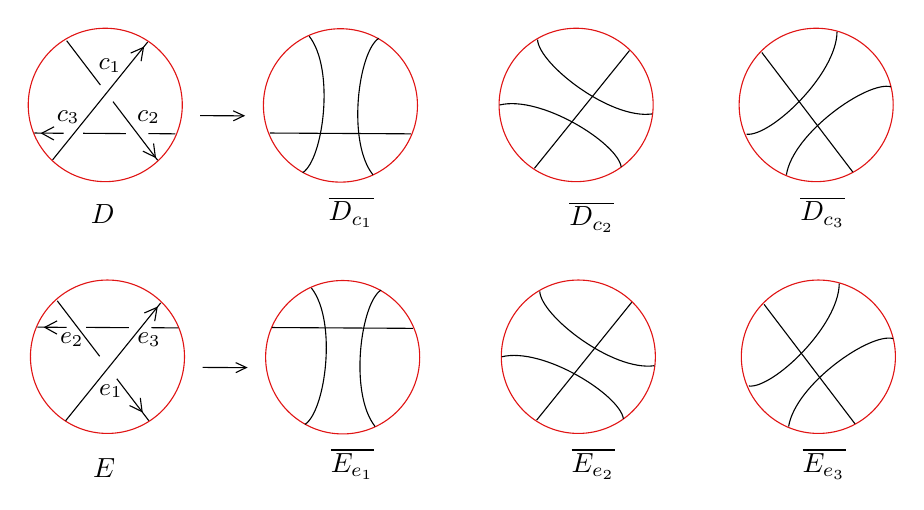
\begin{tikzpicture}[x=0.75pt,y=0.75pt,yscale=-0.8,xscale=0.8]
				\draw  [color={rgb, 255:red, 224; green, 20; blue, 20 }  ,draw opacity=1 ] (179.08,413.14) .. controls (179.08,387.63) and (199.85,366.94) .. (225.47,366.94) .. controls (251.09,366.94) and (271.86,387.63) .. (271.86,413.14) .. controls (271.86,438.65) and (251.09,459.33) .. (225.47,459.33) .. controls (199.85,459.33) and (179.08,438.65) .. (179.08,413.14) -- cycle ;
				\draw  [color={rgb, 255:red, 224; green, 20; blue, 20 }  ,draw opacity=1 ] (37.44,412.85) .. controls (37.44,387.33) and (58.21,366.65) .. (83.83,366.65) .. controls (109.45,366.65) and (130.22,387.33) .. (130.22,412.85) .. controls (130.22,438.36) and (109.45,459.04) .. (83.83,459.04) .. controls (58.21,459.04) and (37.44,438.36) .. (37.44,412.85) -- cycle ;
				\draw   (52.92,433.95) -- (45.6,429.89) -- (53.02,426) ;
				\draw    (142.41,570.92) -- (168.81,571.06) ;
				\draw   (162.38,568.03) -- (168.78,570.98) -- (162.43,574.05) ;
				\draw  [color={rgb, 255:red, 224; green, 20; blue, 20 }  ,draw opacity=1 ] (321.01,412.85) .. controls (321.01,387.33) and (341.78,366.65) .. (367.41,366.65) .. controls (393.03,366.65) and (413.8,387.33) .. (413.8,412.85) .. controls (413.8,438.36) and (393.03,459.04) .. (367.41,459.04) .. controls (341.78,459.04) and (321.01,438.36) .. (321.01,412.85) -- cycle ;
				\draw    (394.56,450.22) .. controls (392.44,435.85) and (346.12,406.79) .. (321.29,412.88) ;
				\draw  [color={rgb, 255:red, 224; green, 20; blue, 20 }  ,draw opacity=1 ] (465.58,412.85) .. controls (465.58,387.33) and (486.35,366.65) .. (511.97,366.65) .. controls (537.59,366.65) and (558.36,387.33) .. (558.36,412.85) .. controls (558.36,438.36) and (537.59,459.04) .. (511.97,459.04) .. controls (486.35,459.04) and (465.58,438.36) .. (465.58,412.85) -- cycle ;
				\draw    (556.95,401.89) .. controls (542.88,398.25) and (498.09,429.62) .. (494.05,454.87) ;
				\draw    (52.14,445.9) -- (109.38,374.96) ;
				\draw    (60.58,374.16) -- (80.9,400.84) ;
				\draw    (88.5,410.86) -- (115.38,446.16) ;
				\draw    (41.11,429.76) -- (58.74,429.92) ;
				\draw    (70.46,429.92) -- (96.28,430.1) ;
				\draw    (109.74,430.1) -- (126.09,430.25) ;
				\draw   (112.93,436.05) -- (114.01,444.35) -- (106.47,440.69) ;
				\draw   (99.15,381.6) -- (106.82,378.24) -- (105.4,386.5) ;
				\draw    (182.91,429.76) -- (267.89,430.25) ;
				\draw    (248.56,372.71) .. controls (236.36,380.6) and (229.15,434.81) .. (245.01,454.87) ;
				\draw    (202.77,453.6) .. controls (215,445.75) and (222.42,391.58) .. (206.65,371.45) ;
				\draw    (342.3,451.01) -- (399.55,380.08) ;
				\draw    (344.18,373.51) .. controls (344.79,388.03) and (387.85,421.75) .. (413.18,418.26) ;
				\draw    (479.25,381.27) -- (534.05,453.27) ;
				\draw    (470.15,430.49) .. controls (484.6,432.01) and (524.26,394.37) .. (524.53,368.8) ;
				\draw  [color={rgb, 255:red, 224; green, 20; blue, 20 }  ,draw opacity=1 ] (180.41,564.78) .. controls (180.41,539.27) and (201.18,518.58) .. (226.8,518.58) .. controls (252.43,518.58) and (273.2,539.27) .. (273.2,564.78) .. controls (273.2,590.29) and (252.43,610.98) .. (226.8,610.98) .. controls (201.18,610.98) and (180.41,590.29) .. (180.41,564.78) -- cycle ;
				\draw  [color={rgb, 255:red, 224; green, 20; blue, 20 }  ,draw opacity=1 ] (38.77,564.49) .. controls (38.77,538.98) and (59.54,518.29) .. (85.16,518.29) .. controls (110.78,518.29) and (131.55,538.98) .. (131.55,564.49) .. controls (131.55,590) and (110.78,610.68) .. (85.16,610.68) .. controls (59.54,610.68) and (38.77,590) .. (38.77,564.49) -- cycle ;
				\draw   (54.75,550.84) -- (47.43,546.78) -- (54.86,542.89) ;
				\draw    (140.92,419.28) -- (167.32,419.42) ;
				\draw   (160.88,416.39) -- (167.29,419.34) -- (160.94,422.41) ;
				\draw  [color={rgb, 255:red, 224; green, 20; blue, 20 }  ,draw opacity=1 ] (322.35,564.49) .. controls (322.35,538.98) and (343.12,518.29) .. (368.74,518.29) .. controls (394.36,518.29) and (415.13,538.98) .. (415.13,564.49) .. controls (415.13,590) and (394.36,610.68) .. (368.74,610.68) .. controls (343.12,610.68) and (322.35,590) .. (322.35,564.49) -- cycle ;
				\draw    (395.89,601.87) .. controls (393.78,587.49) and (347.45,558.43) .. (322.62,564.52) ;
				\draw  [color={rgb, 255:red, 224; green, 20; blue, 20 }  ,draw opacity=1 ] (466.91,564.49) .. controls (466.91,538.98) and (487.68,518.29) .. (513.31,518.29) .. controls (538.93,518.29) and (559.7,538.98) .. (559.7,564.49) .. controls (559.7,590) and (538.93,610.68) .. (513.31,610.68) .. controls (487.68,610.68) and (466.91,590) .. (466.91,564.49) -- cycle ;
				\draw    (558.28,553.54) .. controls (544.21,549.89) and (499.42,581.26) .. (495.38,606.51) ;
				\draw    (59.97,603.02) -- (117.22,532.08) ;
				\draw    (54.92,530.81) -- (80.45,564.18) ;
				\draw    (90.8,577.76) -- (110.07,603) ;
				\draw    (42.94,546.65) -- (60.57,546.81) ;
				\draw    (72.3,546.81) -- (98.11,546.99) ;
				\draw    (111.57,546.99) -- (127.92,547.14) ;
				\draw   (104.93,589.25) -- (106.01,597.55) -- (98.47,593.89) ;
				\draw   (107.37,538.13) -- (115.04,534.78) -- (113.63,543.03) ;
				\draw    (184.24,546.9) -- (269.22,547.39) ;
				\draw    (249.89,524.35) .. controls (237.69,532.24) and (230.48,586.45) .. (246.34,606.51) ;
				\draw    (204.1,605.24) .. controls (216.33,597.4) and (223.76,543.22) .. (207.98,523.09) ;
				\draw    (343.64,602.66) -- (400.88,531.72) ;
				\draw    (345.52,525.16) .. controls (346.13,539.67) and (389.18,573.39) .. (414.51,569.9) ;
				\draw    (480.58,532.92) -- (535.38,604.92) ;
				\draw    (471.48,582.13) .. controls (485.94,583.66) and (525.6,546.01) .. (525.86,520.44) ;
				\draw (216.75,466.43) node [anchor=north west][inner sep=0.75pt]    {$\overline{D_{c_{1}}}$};
				\draw (73.6,471.3) node [anchor=north west][inner sep=0.75pt]    {$D$};
				\draw (361.79,469.43) node [anchor=north west][inner sep=0.75pt]    {$\overline{D_{c_{2}{}}}$};
				\draw (500.82,466.43) node [anchor=north west][inner sep=0.75pt]    {$\overline{D_{c_{3}}}$};
				\draw (78.2,383.54) node [anchor=north west][inner sep=0.75pt]  [font=\small]  {$c_{1}$};
				\draw (101.5,414.54) node [anchor=north west][inner sep=0.75pt]  [font=\small]  {$c_{2}$};
				\draw (53.1,414.54) node [anchor=north west][inner sep=0.75pt]  [font=\small]  {$c_{3}$};
				\draw (218.08,618.07) node [anchor=north west][inner sep=0.75pt]    {$\overline{E_{e_{1}}}$};
				\draw (74.93,624.07) node [anchor=north west][inner sep=0.75pt]    {$E$};
				\draw (363.13,618.07) node [anchor=north west][inner sep=0.75pt]    {$\overline{E_{e_{2}{}}}$};
				\draw (502.16,618.07) node [anchor=north west][inner sep=0.75pt]    {$\overline{E_{e_{3}}}$};
				\draw (78.58,579.57) node [anchor=north west][inner sep=0.75pt]  [font=\small]  {$e_{1}$};
				\draw (55,548.6) node [anchor=north west][inner sep=0.75pt]  [font=\small]  {$e_{2}$};
				\draw (101.57,548.6) node [anchor=north west][inner sep=0.75pt]  [font=\small]  {$e_{3}$};			
			\end{tikzpicture}
			\caption{$0$-smoothing and flattening related to $\Omega_3$.} \label{fig17}
		\end{center}
	\end{figure} 
	
	Therefore, 
	\begin{eqnarray*}
		\mathcal{F} (D) & = & \sum_c w_D(c) \, [\overline{D_c}] - w(D) \, [\overline{D}] \\
		& = & \sum_{ c \notin \{c_1, c_2, c_3 \}} w_D (c) \, [\overline{D_c}] + w_D(c_1) \, [\overline{D_{c_1}}] + w_D (c_2) \, [\overline{D_{c_2}}] + w_D(c_3) \, [\overline{D_{c_3}}] - w (D) \, [\overline{D}] ,
	\end{eqnarray*}
	
	and
	\begin{eqnarray*} 
		\mathcal{F} (E) &=&  \sum_c w_E (c) \, [\overline{E_c}] - w(E) \, [\overline{E}] \\ 
		&=& \sum_{c \notin \{e_1, e_2, e_3 \}} w_E(c) \, [\overline{E_c}] + w_E(e_1) \, [\overline{E_{e_1}}] + w_E(e_2) \, [\overline{E_{e_2}}]  + w_E(e_3) \, [\overline{E_{e_3}}] - w (E) \, [\overline{E}] \\ 
		&=& \sum_{c \notin \{c_1, c_2, c_3\}} w_D (c) \, [\overline{D_c}] + w_D(c_1) \, [\overline{D_{c_1}}] + w_D(c_2) \, [\overline{D_{c_2}}] + w_D(c_3) \, [\overline{D_{c_3}}] - w (D) \, [\overline{D}]   
		= \mathcal{F} (D),
	\end{eqnarray*}
	
	
	(4) $\Omega^{m}_3$-move.  
	Let $D$ and $E$ be virtual knotoid diagrams related by an $\Omega^{m}_3$-move, and $c_* \in D$  a classical crossing involved in  $\Omega^{m}_3$. Denote by $e_*$ the corresponding classical crossing in $E$.  It is clear, see Fig.~\ref{fig18}, that $[\overline{E_{e_*}}] = [\overline{D_{c_*}}]$ and  $w_E(e_*)=w_D(c_*)$. Moreover, $[\overline{E}] = [\overline{D}]$ and $w(E)=w(D)$. Notice that $w_D(c)=w_E(c)$ and $[\overline{E_c}] = [\overline{D_c}]$ if $c$ is a classical crossing not involved in $\Omega^{m}_3$. Therefore,  $\mathcal{F} (E) = \mathcal{F} (D)$.
	
	\begin{figure}[!htb]
		\begin{center}
			\tikzset{every picture/.style={line width=1.0pt}} 
			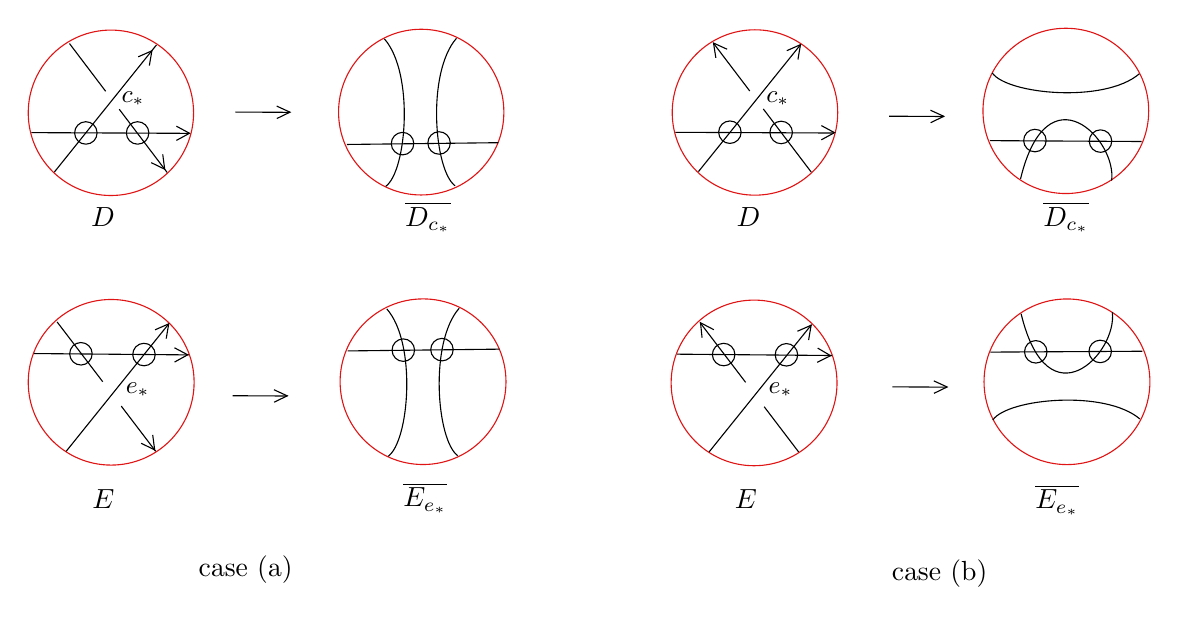
\begin{tikzpicture}[x=0.75pt,y=0.75pt,yscale=-1,xscale=1]
				\draw  [color={rgb, 255:red, 224; green, 20; blue, 20 }  ,draw opacity=1 ] (60.17,1339.57) .. controls (60.17,1317.56) and (78,1299.72) .. (100,1299.72) .. controls (122,1299.72) and (139.83,1317.56) .. (139.83,1339.57) .. controls (139.83,1361.58) and (122,1379.42) .. (100,1379.42) .. controls (78,1379.42) and (60.17,1361.58) .. (60.17,1339.57) -- cycle ;
				\draw   (131.55,1346.02) -- (137.88,1349.43) -- (131.56,1352.87) ;
				\draw    (72.79,1368.08) -- (121.94,1306.89) ;
				\draw    (80.04,1306.2) -- (97.48,1329.21) ;
				\draw    (104.01,1337.85) -- (127.09,1368.31) ;
				\draw   (124.98,1359.58) -- (125.91,1366.74) -- (119.44,1363.59) ;
				\draw   (113.15,1312.61) -- (119.74,1309.72) -- (118.52,1316.84) ;
				\draw  [color={rgb, 255:red, 224; green, 20; blue, 20 }  ,draw opacity=1 ] (520.67,1469.16) .. controls (520.67,1447.12) and (538.56,1429.26) .. (560.63,1429.26) .. controls (582.7,1429.26) and (600.59,1447.12) .. (600.59,1469.16) .. controls (600.59,1491.19) and (582.7,1509.06) .. (560.63,1509.06) .. controls (538.56,1509.06) and (520.67,1491.19) .. (520.67,1469.16) -- cycle ;
				\draw  [color={rgb, 255:red, 224; green, 20; blue, 20 }  ,draw opacity=1 ] (60.17,1469.41) .. controls (60.17,1447.37) and (78.06,1429.51) .. (100.13,1429.51) .. controls (122.2,1429.51) and (140.09,1447.37) .. (140.09,1469.41) .. controls (140.09,1491.44) and (122.2,1509.3) .. (100.13,1509.3) .. controls (78.06,1509.3) and (60.17,1491.44) .. (60.17,1469.41) -- cycle ;
				\draw   (130.63,1452.79) -- (137.01,1456.16) -- (130.69,1459.65) ;
				\draw    (474.92,1341.21) -- (501.32,1341.35) ;
				\draw   (494.88,1338.33) -- (501.29,1341.27) -- (494.94,1344.34) ;
				\draw    (78.43,1502.69) -- (127.74,1441.42) ;
				\draw    (74.07,1440.32) -- (96.07,1469.14) ;
				\draw    (104.98,1480.87) -- (121.58,1502.67) ;
				\draw   (120.15,1494.79) -- (121.09,1501.96) -- (114.59,1498.8) ;
				\draw   (121.26,1444.14) -- (127.86,1441.25) -- (126.65,1448.38) ;
				\draw    (61.68,1349.12) -- (137.93,1349.47) ;
				\draw    (62.92,1455.56) -- (137.53,1456.21) ;
				\draw  [color={rgb, 255:red, 224; green, 20; blue, 20 }  ,draw opacity=1 ] (209.69,1339.24) .. controls (209.69,1317.19) and (227.52,1299.32) .. (249.51,1299.32) .. controls (271.5,1299.32) and (289.33,1317.19) .. (289.33,1339.24) .. controls (289.33,1361.28) and (271.5,1379.16) .. (249.51,1379.16) .. controls (227.52,1379.16) and (209.69,1361.28) .. (209.69,1339.24) -- cycle ;
				\draw  [color={rgb, 255:red, 224; green, 20; blue, 20 }  ,draw opacity=1 ] (370.44,1339.42) .. controls (370.44,1317.42) and (388.29,1299.58) .. (410.31,1299.58) .. controls (432.33,1299.58) and (450.18,1317.42) .. (450.18,1339.42) .. controls (450.18,1361.42) and (432.33,1379.25) .. (410.31,1379.25) .. controls (388.29,1379.25) and (370.44,1361.42) .. (370.44,1339.42) -- cycle ;
				\draw   (442.29,1345.73) -- (448.63,1349.14) -- (442.3,1352.58) ;
				\draw    (383.07,1367.92) -- (432.27,1306.75) ;
				\draw    (390.33,1306.06) -- (407.79,1329.06) ;
				\draw    (414.32,1337.7) -- (437.43,1368.15) ;
				\draw   (391.46,1313.1) -- (390.34,1305.97) -- (396.9,1308.95) ;
				\draw   (425.64,1309.64) -- (432.23,1306.75) -- (431.02,1313.87) ;
				\draw  [color={rgb, 255:red, 224; green, 20; blue, 20 }  ,draw opacity=1 ] (210.43,1469.13) .. controls (210.43,1447.09) and (228.32,1429.23) .. (250.39,1429.23) .. controls (272.46,1429.23) and (290.35,1447.09) .. (290.35,1469.13) .. controls (290.35,1491.16) and (272.46,1509.03) .. (250.39,1509.03) .. controls (228.32,1509.03) and (210.43,1491.16) .. (210.43,1469.13) -- cycle ;
				\draw  [color={rgb, 255:red, 224; green, 20; blue, 20 }  ,draw opacity=1 ] (369.92,1469.71) .. controls (369.92,1447.68) and (387.81,1429.81) .. (409.88,1429.81) .. controls (431.95,1429.81) and (449.84,1447.68) .. (449.84,1469.71) .. controls (449.84,1491.74) and (431.95,1509.61) .. (409.88,1509.61) .. controls (387.81,1509.61) and (369.92,1491.74) .. (369.92,1469.71) -- cycle ;
				\draw   (440.54,1452.94) -- (446.75,1456.6) -- (440.29,1459.8) ;
				\draw    (159.92,1339.21) -- (186.32,1339.35) ;
				\draw   (179.88,1336.33) -- (186.29,1339.27) -- (179.94,1342.34) ;
				\draw    (388.19,1502.99) -- (437.49,1441.72) ;
				\draw    (383.83,1440.62) -- (405.82,1469.45) ;
				\draw    (414.74,1481.17) -- (431.34,1502.97) ;
				\draw   (384.82,1447.93) -- (384.08,1440.74) -- (390.49,1444.07) ;
				\draw   (430.76,1444.82) -- (437.37,1441.92) -- (436.15,1449.05) ;
				\draw   (392.81,1348.92) .. controls (392.81,1345.92) and (395.24,1343.5) .. (398.23,1343.5) .. controls (401.22,1343.5) and (403.65,1345.92) .. (403.65,1348.92) .. controls (403.65,1351.91) and (401.22,1354.33) .. (398.23,1354.33) .. controls (395.24,1354.33) and (392.81,1351.91) .. (392.81,1348.92) -- cycle ;
				\draw   (417.51,1349.04) .. controls (417.51,1346.05) and (419.94,1343.62) .. (422.93,1343.62) .. controls (425.92,1343.62) and (428.35,1346.05) .. (428.35,1349.04) .. controls (428.35,1352.03) and (425.92,1354.46) .. (422.93,1354.46) .. controls (419.94,1354.46) and (417.51,1352.03) .. (417.51,1349.04) -- cycle ;
				\draw    (371.95,1348.97) -- (448.27,1349.31) ;
				\draw    (372.8,1455.86) -- (447.41,1456.51) ;
				\draw  [color={rgb, 255:red, 224; green, 20; blue, 20 }  ,draw opacity=1 ] (520.16,1338.65) .. controls (520.16,1316.67) and (538.03,1298.84) .. (560.08,1298.84) .. controls (582.14,1298.84) and (600.01,1316.67) .. (600.01,1338.65) .. controls (600.01,1360.64) and (582.14,1378.47) .. (560.08,1378.47) .. controls (538.03,1378.47) and (520.16,1360.64) .. (520.16,1338.65) -- cycle ;
				\draw    (523.45,1352.98) -- (596.59,1353.4) ;
				\draw    (582.15,1372.25) .. controls (584.73,1352.43) and (551.17,1317.95) .. (538.26,1371.39) ;
				\draw    (524.66,1320.4) .. controls (531.84,1330.65) and (578.69,1335.12) .. (595.44,1320.82) ;
				\draw    (286.64,1353.97) -- (213.7,1354.83) ;
				\draw    (232.42,1375.01) .. controls (242.53,1367.64) and (246.26,1320.54) .. (231.77,1303.95) ; 
				\draw   (245.93,1354.33) .. controls (245.98,1357.32) and (243.6,1359.79) .. (240.6,1359.84) .. controls (237.61,1359.89) and (235.14,1357.51) .. (235.09,1354.52) .. controls (235.04,1351.52) and (237.42,1349.06) .. (240.42,1349) .. controls (243.41,1348.95) and (245.88,1351.33) .. (245.93,1354.33) -- cycle ;
				\draw   (258.2,1359.53) .. controls (255.21,1359.57) and (252.74,1357.18) .. (252.7,1354.19) .. controls (252.65,1351.2) and (255.04,1348.74) .. (258.03,1348.69) .. controls (261.03,1348.65) and (263.49,1351.03) .. (263.53,1354.03) .. controls (263.58,1357.02) and (261.19,1359.48) .. (258.2,1359.53) -- cycle ;
				\draw    (265.84,1374.74) .. controls (255.73,1367.37) and (252,1320.27) .. (266.49,1303.68) ;
				\draw    (523.72,1454.87) -- (596.92,1454.45) ;
				\draw    (582.47,1435.56) .. controls (585.05,1455.42) and (551.46,1489.97) .. (538.54,1436.42) ;
				\draw    (524.93,1487.52) .. controls (532.12,1477.24) and (579.01,1472.77) .. (595.77,1487.1) ;
				\draw    (287.26,1453.44) -- (214.07,1454.3) ;
				\draw    (233.59,1505.07) .. controls (243.73,1497.71) and (247.48,1450.63) .. (232.93,1434.05) ;
				\draw    (267.12,1504.79) .. controls (256.98,1497.43) and (253.24,1450.36) .. (267.78,1433.77) ;
				\draw   (88.02,1354.69) .. controls (85.03,1354.74) and (82.56,1352.35) .. (82.52,1349.36) .. controls (82.47,1346.37) and (84.86,1343.9) .. (87.85,1343.86) .. controls (90.85,1343.81) and (93.31,1346.2) .. (93.35,1349.19) .. controls (93.4,1352.19) and (91.01,1354.65) .. (88.02,1354.69) -- cycle ;
				\draw   (112.95,1354.69) .. controls (109.96,1354.74) and (107.5,1352.35) .. (107.45,1349.36) .. controls (107.41,1346.37) and (109.79,1343.9) .. (112.79,1343.86) .. controls (115.78,1343.81) and (118.24,1346.2) .. (118.29,1349.19) .. controls (118.33,1352.19) and (115.94,1354.65) .. (112.95,1354.69) -- cycle ;
				\draw   (545.27,1358.36) .. controls (542.28,1358.41) and (539.82,1356.02) .. (539.77,1353.02) .. controls (539.73,1350.03) and (542.12,1347.57) .. (545.11,1347.52) .. controls (548.1,1347.48) and (550.56,1349.87) .. (550.61,1352.86) .. controls (550.65,1355.85) and (548.26,1358.31) .. (545.27,1358.36) -- cycle ;
				\draw   (576.87,1358.63) .. controls (573.88,1358.67) and (571.42,1356.28) .. (571.37,1353.29) .. controls (571.33,1350.3) and (573.72,1347.84) .. (576.71,1347.79) .. controls (579.7,1347.75) and (582.16,1350.13) .. (582.21,1353.13) .. controls (582.25,1356.12) and (579.86,1358.58) .. (576.87,1358.63) -- cycle ;
				\draw    (158.59,1475.88) -- (184.99,1476.02) ;
				\draw   (178.55,1472.99) -- (184.96,1475.94) -- (178.61,1479.01) ;
				\draw    (476.52,1471.61) -- (502.92,1471.75) ;
				\draw   (496.48,1468.73) -- (502.89,1471.67) -- (496.54,1474.74) ;
				\draw   (545.68,1460.15) .. controls (542.69,1460.2) and (540.23,1457.81) .. (540.18,1454.82) .. controls (540.14,1451.82) and (542.53,1449.36) .. (545.52,1449.32) .. controls (548.51,1449.27) and (550.97,1451.66) .. (551.02,1454.65) .. controls (551.07,1457.64) and (548.68,1460.11) .. (545.68,1460.15) -- cycle ;
				\draw   (576.72,1459.96) .. controls (573.73,1460.01) and (571.27,1457.62) .. (571.22,1454.63) .. controls (571.18,1451.64) and (573.57,1449.17) .. (576.56,1449.13) .. controls (579.55,1449.08) and (582.01,1451.47) .. (582.06,1454.46) .. controls (582.11,1457.46) and (579.72,1459.92) .. (576.72,1459.96) -- cycle ;
				\draw   (85.64,1461.09) .. controls (82.65,1461.13) and (80.19,1458.75) .. (80.14,1455.75) .. controls (80.1,1452.76) and (82.49,1450.3) .. (85.48,1450.25) .. controls (88.47,1450.21) and (90.93,1452.6) .. (90.98,1455.59) .. controls (91.02,1458.58) and (88.64,1461.04) .. (85.64,1461.09) -- cycle ;
				\draw   (116.02,1461.46) .. controls (113.03,1461.51) and (110.56,1459.12) .. (110.52,1456.13) .. controls (110.47,1453.14) and (112.86,1450.67) .. (115.85,1450.63) .. controls (118.85,1450.58) and (121.31,1452.97) .. (121.35,1455.96) .. controls (121.4,1458.96) and (119.01,1461.42) .. (116.02,1461.46) -- cycle ;
				\draw   (259.59,1459.09) .. controls (256.6,1459.13) and (254.13,1456.75) .. (254.09,1453.75) .. controls (254.04,1450.76) and (256.43,1448.3) .. (259.42,1448.25) .. controls (262.42,1448.21) and (264.88,1450.6) .. (264.92,1453.59) .. controls (264.97,1456.58) and (262.58,1459.04) .. (259.59,1459.09) -- cycle ;
				\draw   (240.96,1459.34) .. controls (237.97,1459.38) and (235.51,1457) .. (235.46,1454) .. controls (235.42,1451.01) and (237.81,1448.55) .. (240.8,1448.5) .. controls (243.79,1448.46) and (246.25,1450.85) .. (246.3,1453.84) .. controls (246.34,1456.83) and (243.95,1459.29) .. (240.96,1459.34) -- cycle ;
				\draw   (425.55,1461.59) .. controls (422.56,1461.63) and (420.1,1459.25) .. (420.05,1456.25) .. controls (420.01,1453.26) and (422.4,1450.8) .. (425.39,1450.75) .. controls (428.38,1450.71) and (430.84,1453.1) .. (430.89,1456.09) .. controls (430.93,1459.08) and (428.55,1461.54) .. (425.55,1461.59) -- cycle ;
				\draw   (395.3,1461.46) .. controls (392.31,1461.51) and (389.85,1459.12) .. (389.8,1456.13) .. controls (389.76,1453.14) and (392.15,1450.67) .. (395.14,1450.63) .. controls (398.13,1450.58) and (400.59,1452.97) .. (400.64,1455.96) .. controls (400.68,1458.96) and (398.3,1461.42) .. (395.3,1461.46) -- cycle ;
				\draw (89.15,1383.96) node [anchor=north west][inner sep=0.75pt]    {$D$};
				\draw (103.91,1328.07) node [anchor=north west][inner sep=0.75pt]  [font=\small]  {$c_{*}$};
				\draw (105.92,1468.3) node [anchor=north west][inner sep=0.75pt]  [font=\small]  {$e_{*}$};
				\draw (240.54,1381.1) node [anchor=north west][inner sep=0.75pt]    {$\overline{D_{c_{*}}}$};
				\draw (400.17,1383.96) node [anchor=north west][inner sep=0.75pt]    {$D$};
				\draw (414.56,1328.07) node [anchor=north west][inner sep=0.75pt]  [font=\small]  {$c_{*}$};
				\draw (415.68,1468.3) node [anchor=north west][inner sep=0.75pt]  [font=\small]  {$e_{*}$};
				\draw (141,1551.9) node [anchor=north west][inner sep=0.75pt]    {case (a)};
				\draw (475,1553.67) node [anchor=north west][inner sep=0.75pt]    {case (b)};
				\draw (548.04,1381.1) node [anchor=north west][inner sep=0.75pt]    {$\overline{D_{c_{*}}}$};
				\draw (89.82,1519.79) node [anchor=north west][inner sep=0.75pt]    {$E$};
				\draw (239.7,1516.43) node [anchor=north west][inner sep=0.75pt]    {$\overline{E_{e_{*}}{}}$};
				\draw (399.33,1519.79) node [anchor=north west][inner sep=0.75pt]    {$E$};
				\draw (544.2,1517.43) node [anchor=north west][inner sep=0.75pt]    {$\overline{E_{e_{*}}}$};		
			\end{tikzpicture}
			\caption{$0$-smoothing and flattening related to $\Omega_3^{m}$.} \label{fig18}
		\end{center}
	\end{figure} 	
Thus, $\mathcal{F} (D)$ is a virtual knotoid invariant. 
\end{proof}

\end{document}
